\subsection{Relational games}\label{ssec:exp_relational_games}

The \textit{relational games} dataset was contributed as a benchmark for relational reasoning by~\citep{shanahanExplicitlyRelationalNeural}. It consists of a family of binary classification tasks for identifying abstract relational rules between a set of objects represented as images. The objects consist of three sets of simple geometric shapes, referred to as ``pentominoes'', ``hexominoes'', and ``stripes''. The objects are arranged in a $3 \times 3$ grid. Each task corresponds to some relationship between the objects, and the target is to classify whether the relationship holds among a given set of objects or not (see~\Cref{fig:relational_games_dataset}).

In our experiments, we evaluate out-of-distribution generalization by training all models on the pentominoes objects and evaluating on the hexominoes and stripes objects. The input to all models is presented as a sequence of $9$ objects, each represented as a $12 \times 12 \times 3$ RGB image. In all models, the objects are first processed independently by a CNN with a shared architecture. The processed objects are then passed to the central module of the model. The final prediction is produced by an MLP with a shared architecture. We compare four models: a relational convolutional network (abbreviated RelConvNet), CoRelNet~\citep{kergNeuralArchitecture2022}, PrediNet~\citep{shanahanExplicitlyRelationalNeural}, and a Transformer~\citep{vaswani2017attention}. The pentominoes split is used for training,
% We hold out 1000 samples for validation (during training) and 5000 samples for testing (after training), and use the rest as the training set. \awni{we don't show val or test accs on the pentos objects, so not relevant.}
and the hexominoes and stripes splits are used to test out-of-distribution generalization after training. 
\todo{removed optimizer, loss, etc. putting in appendix. }
% We train for 50 epochs using the categorical cross-entropy loss and the Adam optimizer with learning rate $0.001$, $\beta_1 = 0.9, \beta_2 = 0.999, \epsilon = 10^{-7}$. We use a batch size of 512. For each model and task, we run 5 trials with different random seeds.
\Cref{sec:experiments_supplement} describes further experimental details about the architectures and training setup.

\begin{figure}[t]
    \centering
    \begin{subfigure}[t]{0.37\textwidth}
        \centering
        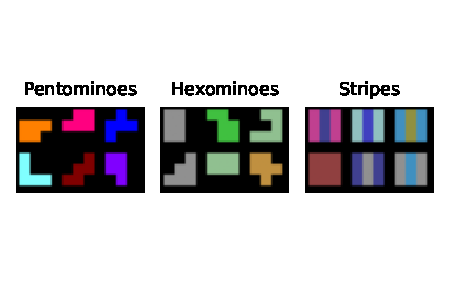
\includegraphics[width=0.99\textwidth]{figs/relational_games_objects.pdf}
        % \caption{Examples of objects from each split.}\label{fig:relational_games_objects}
    \end{subfigure}
    \begin{subfigure}[t]{0.62\textwidth}
        \centering
        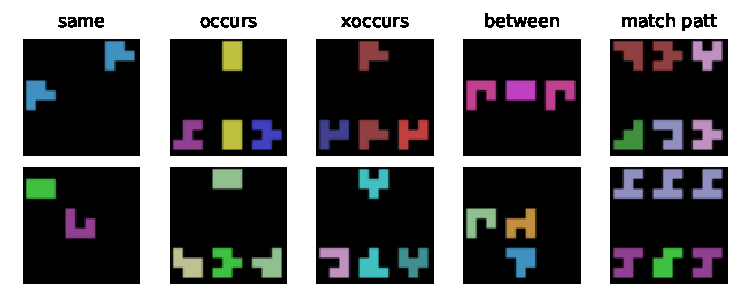
\includegraphics[width=0.95\textwidth]{figs/relational_games_tasks.pdf}
        % \caption{Examples of problem instances for each task. The top row is an example where the relation holds and the bottom row is an example where the relation does not hold.}\label{fig:relational_games_tasks}
    \end{subfigure}
    % \vskip-10pt
    \caption{Relational games dataset.~\textbf{Left} Examples of objects from each split.~\textbf{Right} Examples of problem instances for each task. The first row is an example where the relation holds and the second row is an example where the relation does not hold.}\label{fig:relational_games_dataset}
    % \vskip-12pt
\end{figure}

\textbf{Sample efficiency.} We observe that the relational inductive biases of RelConvNet, and relational models more generally, grant a significant advantage in sample-efficiency.~\Cref{fig:training_curves} shows the training accuracy over the first 2,000 batches for each model. RelConvNet, CoRelNet, and PrediNet are explicitly relational architectures, whereas the Transformer is not. The Transformer is able to process relational information through its attention mechanism, but this information is entangled with the features of individual objects (which, for these relational tasks, is extraneous information). The Transformer consistently requires the largest amount of data to learn the relational games tasks. PrediNet tends to be more sample-efficient. RelConvNet and CoRelNet are the most sample-efficient, with RelConvNet only slightly more sample-efficient on most tasks.

On the `match pattern' task, however, RelConvNet is significantly more sample-efficient. We attribute this to the fact that RelConvNet is able to model higher-order relations through its relational convolution module. The `match pattern' task can be thought of as a second-order relational task---it involves computing the relational pattern in each of two groups, and comparing the two relational patterns. The relational convolution module naturally models this kind of situation since it learns representations of the relational patterns within groups of objects. %The performance we observe here indicates that the relational games dataset is in some sense saturated by models like RelConvNet and CoRelNet and that more complex relational benchmarks are needed to evaluate the limits of these models.

\begin{figure}[t]
    \centering
    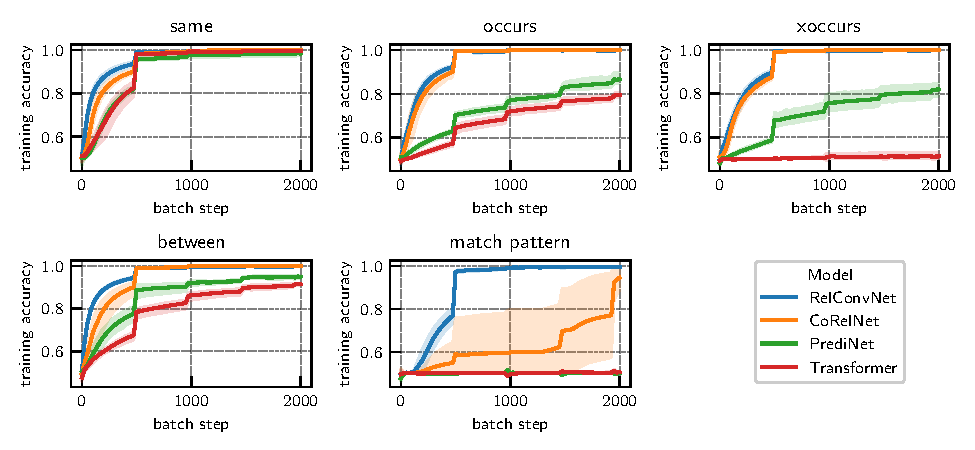
\includegraphics[width=0.95\textwidth]{figs/experiments/all_training_curves.pdf}
    % \vskip-12pt
    \caption{Training curves, up to 2,000 batch steps, for each relational games task. Solid lines indicate the mean over 5 trials and the shaded regions indicate a bootstrap 95\% confidence interval.}\label{fig:training_curves}
    % \vskip-12pt
\end{figure}

\begin{figure}[t]
    \centering
    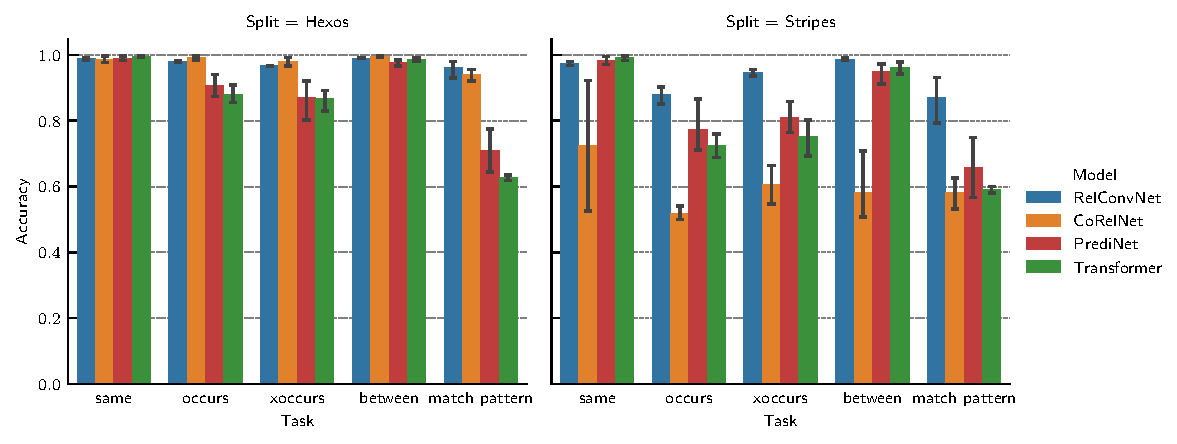
\includegraphics[width=0.95\textwidth]{figs/experiments/relgames_ood_acc.pdf}
    % \vskip-12pt
    \caption{Out-of-distribution generalization on hold-out object sets. Bar heights indicate the mean over 5 trials and the error bars indicate a bootstrap 95\% confidence interval.}\label{fig:ood_generalization}
    % \vskip-15pt
\end{figure}

\textbf{Out-of-distribution generalization.}~\Cref{fig:ood_generalization} reports model performance on the two hold-out object sets after training. On the hexominoes objects, which are similar-looking to the pentominoes objects used for training, RelConvNet and CoRelNet do nearly perfectly. PrediNet and the Transformer do well on the simpler tasks, but struggle with the more difficult `match pattern' task. The `stripes' objects are visually more distinct from the objects in the training split, making generalization more difficult. We observe an overall drop in performance for all models. The drop is particularly dramatic for CoRelNet\footnote{The experiments in \citep{kergNeuralArchitecture2022} on the relational games benchmark use a technique called ``context normalization''~\citep{webbLearningRepresentationsThat2020} as a preprocessing step. We choose not to use this technique since it is an added confounder. We discuss this choice in~\Cref{sec:appendix_tcn_discussion}.}.
% We conjecture that this is due to CoRelNet's inability to model multi-dimensional relations, necessitating that all relational information is squeezed into a scalar quantity. % Or perhaps it's because of the softmax normalization?
The separation between RelConvNet and the other models is largest on the ``match pattern'' task of the stripes split (the most difficult task and the most difficult generalization split). Here, RelConvNet maintains a mean accuracy of 87\% while the other models drop below 65\%. We attribute this to RelConvNet's ability to naturally represent higher-order relations and model groupings of objects.



% \begin{table}
%     \centering
%     \caption{Performance of RelConvNet with group attention on each task.}\label{tab:relgames_groupattn_resuls}
%     \begin{tabular}{lc}
%         \toprule
%         Task & Accuracy \\
%         \midrule
%         same & $0.981 \pm 0.002$\\
%         occurs & $0.949 \pm 0.014$ \\
%         xoccurs & $0.988 \pm 0.004$\\
%         between & $1.000 \pm 0.000$ \\
%         match pattern & $0.987 \pm 0.002$\\
%         \bottomrule
%     \end{tabular}
%     \vskip-10pt
% \end{table}

% \begin{figure}
%     \centering
%         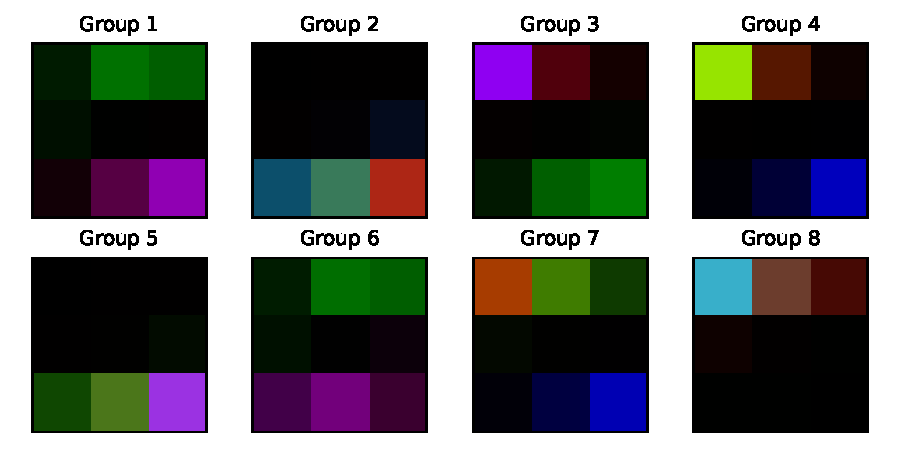
\includegraphics[width=0.65\textwidth]{figs/group_attn_figs/match_patt_group_attn_map.pdf}
%     % \vskip-10pt
%     \caption{Learned groups in the `match pattern' tasks by a 2-layer RelConvNet with group attention.}\label{fig:matchpatt_groupattn}
%     % \vskip-15pt
% \end{figure}


% \todo{removed in-dist accuracy for relconvnet with group attn. the focus of this section is qualitative.}
\textbf{Learning groups via group attention.} Next we analyze RelConvNet's ability to learn useful groupings through group attention in an end-to-end manner. We train a $2$-layer relational convolutional network with $8$ learned groups and a graphlet size of $3$. We group based on position by using positional embeddings for $\mathtt{key}(x_i)$.
% ~\Cref{tab:relgames_groupattn_resuls} shows the in-distribution generalization accuracy achieved by this model on each task. The model is able to learn all tasks.
In~\Cref{fig:matchpatt_groupattn}, we visualize the group attention scores $\alpha_{ij}^g$ (see~\cref{eq:group_attn}) learned from one of the training runs. For each group $g \in [n_g]$, the figure depicts a $3 \times 3$ grid representing the objects attended to in that group. Since each group contains $3$ objects, we represent the value $(\alpha_{ij}^g)_{i \in [3]}$ in the $3$-channel HSV color representation. We observe that 1) group attention learns to ignore the middle row, which contains no relevant information; and 2) the selection of objects in the top row and the bottom row is structured. In particular, group $2$ considers the relational pattern within the bottom row and group $8$ considers the relational pattern in the top row, which is exactly how a human would tackle this problem.

\begin{wrapfigure}{r}{0.5\textwidth}
    \centering
    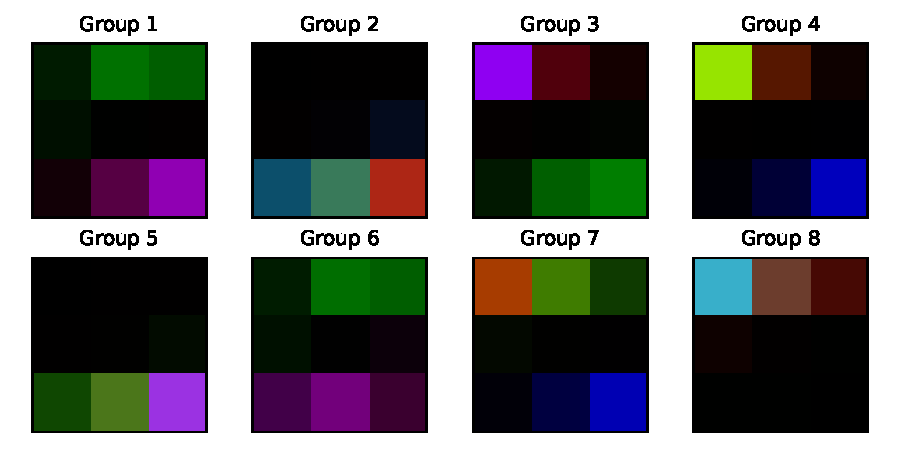
\includegraphics[width=0.5\textwidth]{figs/group_attn_figs/match_patt_group_attn_map.pdf}
    % \vskip-10pt
    \caption{Learned groups in the `match pattern' tasks by a 2-layer RelConvNet with group attention.}\label{fig:matchpatt_groupattn}
    % \vskip-15pt
\end{wrapfigure}